\subsubsection{ボリューム}\label{volume}
\begin{table}[H]
	\begin{tabular}{|p{\colF}|p{\colG}|}	\hline
	名称 & ボリューム(ぼりゅーむ)\\ \hline
	接続箇所 & アナログコネクタ (3pin)\\ \hline
	機能概要 & つまみの回転量を出力\\ \hline
  \end{tabular}
\end{table}

\begin{table}[H]
	\begin{tabular}{|p{\colF}|p{\colG}|}	\hline
	サンプルコードの場所 & 05/anain.hsp\\ \hline
	raspiへの入力 & つまみの回転量 0から1023の値\\ \hline
	raspiへの入力方法 & 力を入れすぎて壊れないよう注意\\ \hline
	raspiからの出力 & なし\\ \hline
	raspiからの出力方法 & なし\\ \hline
  \end{tabular}
\end{table}

\begin{figure}[H]
	\begin{tabular}{|p{\colF}|p{\colG}|} \hline
	使い道 & 音量調整, LEDの明るさ調整, ゲームのコントローラとして\\ \hline
	注意事項 & 強く押して壊さないように注意\\ \hline
	補足 & 先端のつまみをつまんで回転させると抵抗値が変化しraspberry piに入力される電圧が変化します。今回使うボリュームは左に回しきったときは変化が小さく、右に回すほど変化が大きくなります(指数関数的)。この設定をAカーブと呼びます (図\ref{ボリュームの特性})。これはボリュームがしばしば音量調節に利用され、人間の耳の感度は対数関数的(小さい音ほど敏感で大きい音に関しては鈍感)であることからこのように設定されています。もちろん、ボリュームは音量調節以外にも使用されるため、用途に応じて特性が線形(傾きが一定)なBカーブや対数関数的(傾きが小さくなっていく)なCカーブなどが存在します。\par
ボリュームには端子が3つ付いており、図\ref{ボリュームの仕組み}のように1つに+電源を、1つに-電源をつなげ、もう1つを出力として使用します。+電源から-電源までに帯状の抵抗器が接続されており、その間に出力の端子が接続されています。シャフトを回すことで、出力端子の位置が変化し、結果プラス電源端子-出力端子間と出力端子-マイナス電源端子間の抵抗値が変化することになります。
	\begin{minipage}[t]{0.45\linewidth}
    \smallskip
      \centering
      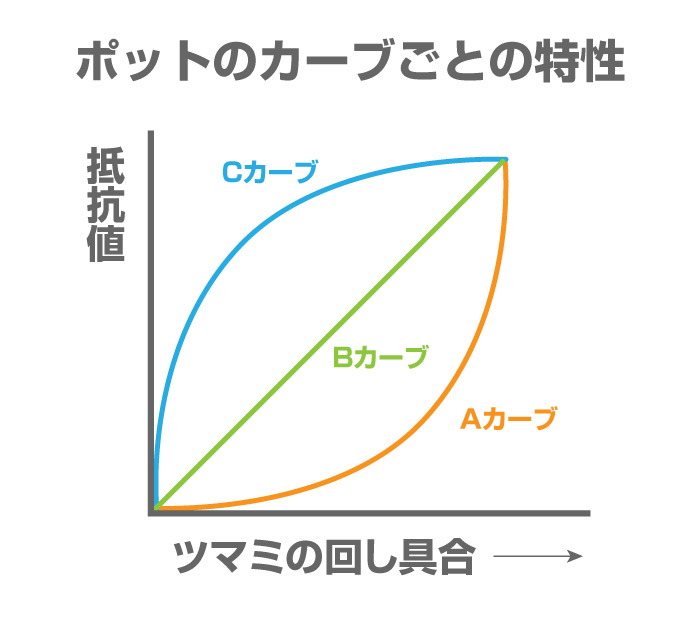
\includegraphics[width=\linewidth]{images/chap05/text05-img050.jpg}
      \caption{ボリュームの特性}
      \label{ボリュームの特性}
      \smallskip
    \end{minipage}
    \begin{minipage}[t]{0.45\linewidth}
    \smallskip
      \centering
      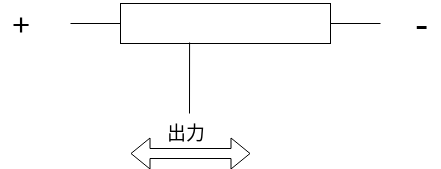
\includegraphics[width=\linewidth]{images/chap05/text05-img051.png}
      \caption{ボリュームの仕組み}
      \label{ボリュームの仕組み}
      \smallskip
    \end{minipage}\\ \hline
  \end{tabular}
\end{figure}

\begin{figure}[H]
	\begin{tabular}{|p{\colH}|p{\colI}|p{\colH}|p{\colI}|} \hline
	外観 & 
	\begin{minipage}[t]{\linewidth}
    \smallskip
      \centering
      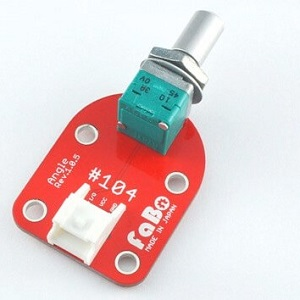
\includegraphics[width=\linewidth]{images/chap05/text05-img022.jpg}
      \caption{ボリューム}
      \smallskip
    \end{minipage} &
    回路記号 & 
    \begin{minipage}[t]{\linewidth}
    \smallskip
      \centering
      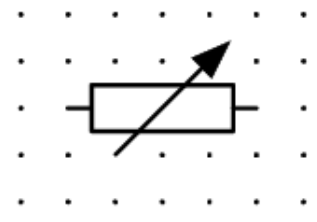
\includegraphics[width=\linewidth]{images/chap05/text05-img052.png}
      \caption{ボリュームの回路図}
      \smallskip
    \end{minipage}\\ \hline
  \end{tabular}
\end{figure}